\documentclass{slides}
\usepackage[english]{babel}
\usepackage{palatino}
\usepackage[dvips]{graphicx}
% pause is very useful for pausing before presenting more of a page of text..
%\usepackage{pause}
\usepackage{color,sshow}

\begin{document}
% set the whole thing in roman
\rm

% this eliminates the footer entirely
\pagestyle{empty}

% play with this if necessary..
\global\parskip .25in

% disable vertical centering
\vfill

% don't hyphenate & flush right on slides!
\raggedright
% if not above, use \sloppy
% \sloppy

\begin{slide}{}
  \stitle{JPEG Specials!}

  \centerline{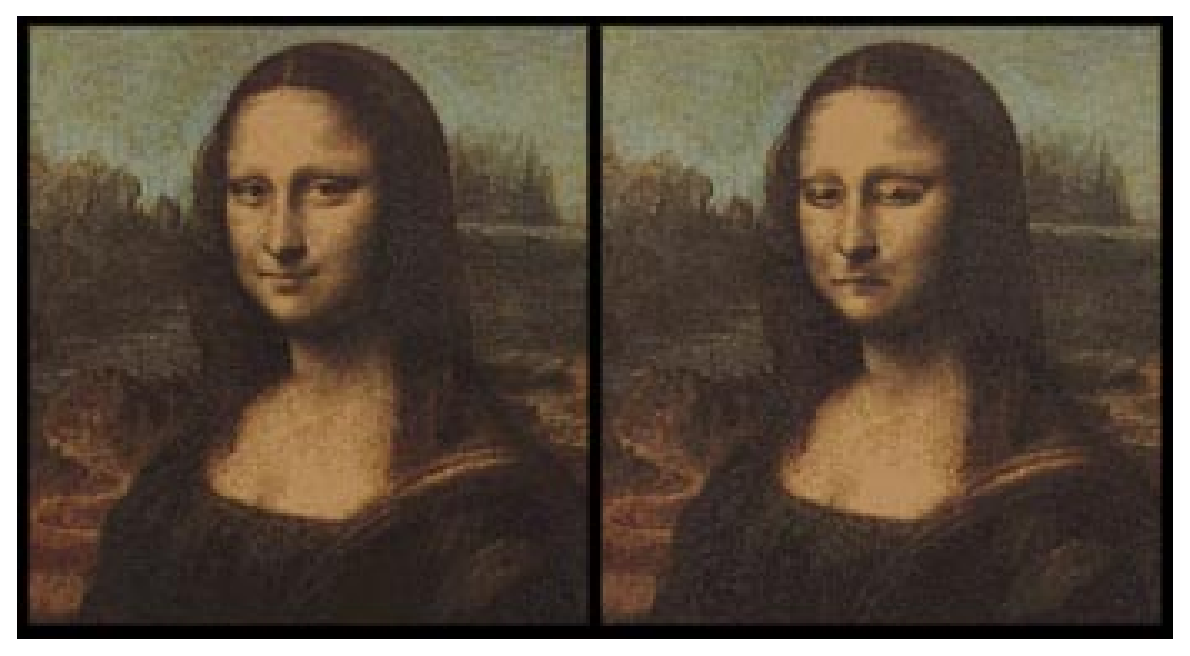
\includegraphics[width=4.5in]{sshow_demo_mona.eps}}
%  \jpegimage{sshow_demo_mona.jpg}

  \vfill
\end{slide}

\begin{slide}{}
  \stitle{This is a Title}

  {\yc This is something important:}  And this is just normal.

  \begin{itemize}
  \item {\rc Point one:} one.
  \item {\gc Point two:} two.
  \item {\mc Point three:} three.
  \end{itemize}

  \vfill
\end{slide}

\begin{slide}{}
  \stitle{This is a Title Also}

  This is how you would include a postscript figure (using same
  fg, bg colors as the regular text):

  \gswb
  \centerline{
\includegraphics[width=6in]{sshow_demo_fig.ps}}

  \vfill
\end{slide}

\begin{slide}{}
  \stitle{This is a Title As Well}

  You can set the foreground and background colors of ps (note
  you need a white background square to get the background to actually
  show up as white):

  \gsbw
  \centerline{
\includegraphics[width=6in]{sshow_demo_fig.ps}}

  \vfill
\end{slide}

\begin{slide}{}
  \stitle{Animations!}

  \href{file:sshow_demo_movie.-300+150.avi}{Animation Demo}

  \vfill
\end{slide}

\end{document}

